\section{Dataset description}
The dataset is provided by the website Kaggle and it contains ride details for the year \num{2020} of the company Citi Bike in the Jersey City area. Citi Bike is a privately owned public bicycle sharing system serving the New York City boroughs of the Bronx, Brooklyn, Manhattan, and Queens, as well as Jersey City, New Jersey. In order to provide an effective analysis, we have collected data relating to the most significant weather variables in the city of New York and we have generated two dummy variables that associate two events with each observation that can influence the analyses, i.e. the presence of public holidays and the presence of lockdowns as in \num{2020} there were restrictions in the city of New York due to the COVID-\num{19} pandemic.
Through a data processing work, we have obtained a dataset that contains the information sampled in discrete time with daily and hourly frequency. Below are some characteristics of the available data.

\subsection{Bike data}
This partition contains all the information relating to the bike rental:
\begin{itemize}
	\item \textbf{pickups counters}: number of rentals of a given station (figure \ref{Trend});
	\item \textbf{mean trip duration}: mean rental time (figure \ref{Trend});
	\item \textbf{mean clients age}: mean age of customers who rent;
	\item \textbf{male counters}: male client number;
	\item \textbf{female counters}: female client number;
	\item \textbf{unknown gender counters}: unknown gender number;
	\item \textbf{subscribers counters}: number of customers who have an annual subscription;
	\item \textbf{customers counters}: number of customers who have \num{4}-hour pass or \num{3}-day pass;
	\item \textbf{distance}: indicates the distance between a rental station and the nearest train or subway station in \unit{\kilo\meter}. (figure \ref{Map})
	
\end{itemize}
All this data is sampled hourly and daily, except for the distance, that is a time-invariant variable, which we have entered by carrying out an in-depth analysis of the means of transport in the area, with the hypothesis that it may influence the demand for rentals.

\begin{figure}[h!]
	\centering
	\subfigure[]{\label{Distances_map}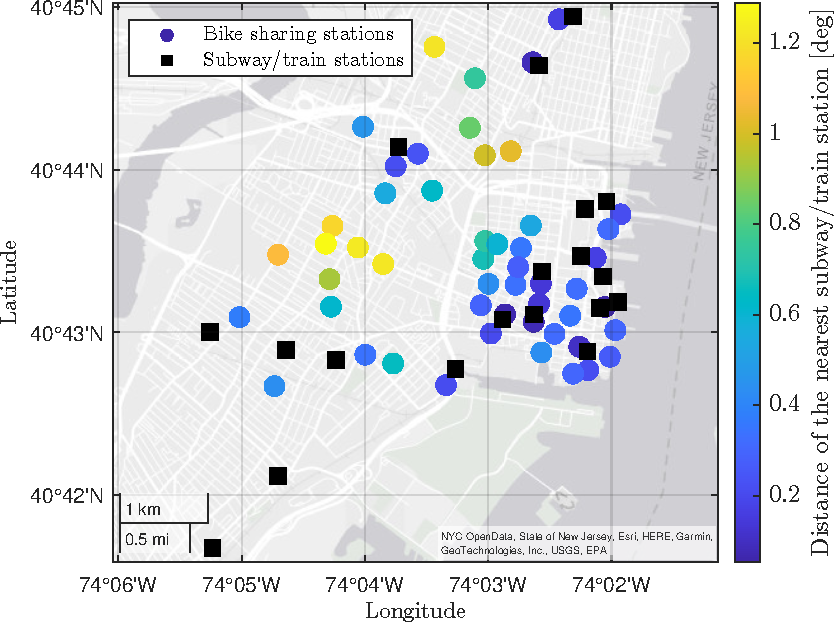
\includegraphics[height=200px]{Images/Dataset description/Chosen/Distances_map}}\quad
	\subfigure[]{\label{Train_map}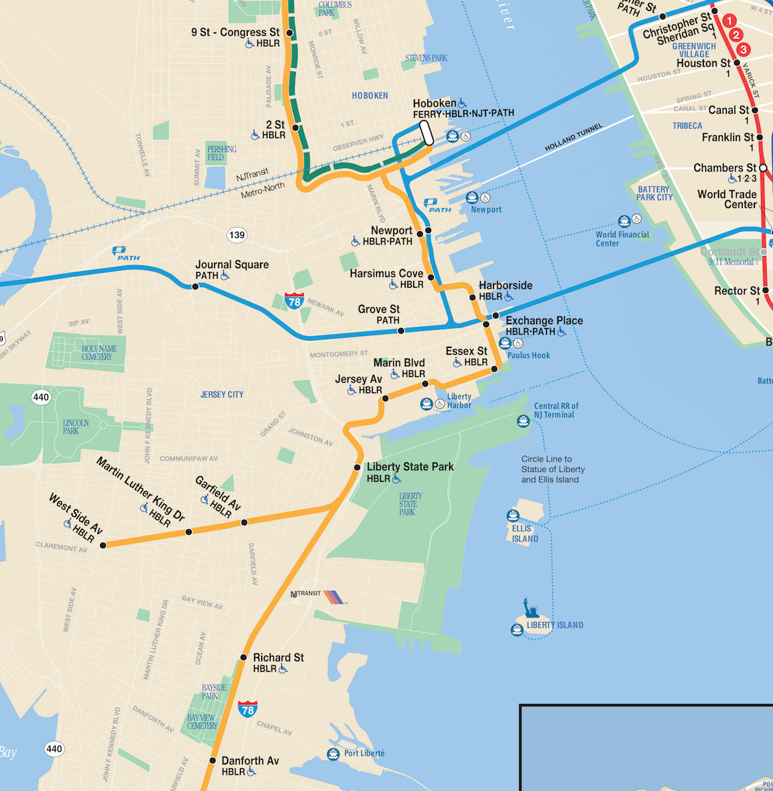
\includegraphics[height=200px]{Images/Dataset description/Chosen/Train_map}}\quad
	\caption[]{the maps summarizes our area of interest. On the left, the black squares indicate the means of transport stations, the dots indicate the bike sharing stations, the colorbar describes the distance from the nearest means of transport station. On the right, it is the public transport map from which we have obtained the coordinates of the main stations, in particular in blue is the route of the path service which reaches Manhattan, in yellow is the NJ transport service which extends over the entire Jersey area.}
\end{figure} 

\subsection{Weather data}
Also in this case the weather variables are sampled in discrete time with daily and hourly frequency and they are thus defined:
\begin{itemize}
	\item \textbf{mean temperature}: in \unit{\degreeCelsius};
	\item \textbf{mean feels-like temperature}: in \unit{\degreeCelsius} (figure \ref{T_plot_box});
	\item \textbf{relative humidity}: in percentage;
	\item \textbf{rainfall}: in \unit{\milli\meter} (figure \ref{Rain_plot_box});
	\item \textbf{snowfall}: in \unit{\centi\meter};
	\item \textbf{mean wind speed}: in \unit{\kilo\meter/\hour};
	\item \textbf{cloud cover}: describes the percentage of covered sky;
	\item \textbf{visibility}: describes the maximum distance of visibility in \unit{\kilo\meter}. In the absence of fog there is a field of vision of \num{16} km;
	\item \textbf{UV index}: indicates the energy of UV rays, with a dimensionless variable ranging from \num{1} to \num{10}.
\end{itemize}
The reason why we have taken into consideration the weather variables is because it's easy to think that the weather can influence a person's choice of rent or not rent a bike. For example, we report two plots that showing how some meteorological variables affect rentals.
\\
\\
\\
\begin{tabular}{|c|c|c|c|c|c|c|c|c|}
	\hline
	\multicolumn{1}{|c|}{\textbf{Variable}} & \textbf{Min} & \textbf{Max} & \textbf{Mean} & \textbf{Median} & \textbf{Std} & \textbf{Skewness}  & 
	\multicolumn{1}{c|}{\textbf{Kurtosis}}\\
	\hline
	\textbf{temperature (°C)} & -3.5 & 30.4 & 14.546 & 14 & 8.49 & 0.042 & 1.855\\
	\hline
	\textbf{feels like temperature} & -7.7 & 33.3 & 13.805 & 13.9 & 9.796 & 0.0405 & 1.958 \\
	\hline
	\textbf{humidity (\%)} & 35.1 & 93.5 & 65.283 & 66.100 & 13.775 & 0.0752 & 2.176 \\
	\hline
	\textbf{rainfall (mm)} & 0 & 31.03 & 1.11 & 0 & 3.44 & 5.44 & 39.01\\
	\hline
	\textbf{snowfall (cm)} & 0 & 157.50 & 0.775 & 0 & 9.61 & 14.45 & 219.19\\
	\hline
	\textbf{windspeed (km/h)} & 9.90 & 47.8 & 20.64 & 19.90 & 6.89 & 0.98 & 3.90\\
	\hline
	\textbf{cloud cover (\%)} & 0.10 & 100 & 39.45 & 37.15 & 29.79 & 0.35 & 1.95\\
	\hline
	\textbf{visibility (km)} & 6.50 & 16 & 15.29 & 16 & 1.54 & -2.99 & 12.83\\
	\hline
	\textbf{UV index'} & 0 & 10 & 5.92 & 6 & 2.88 & -0.21 & 1.84\\
	\hline
	

\end{tabular}
\\
\\
\begin{figure}[h!]
	\centering
	\subfigure[]{\label{T_plot_box}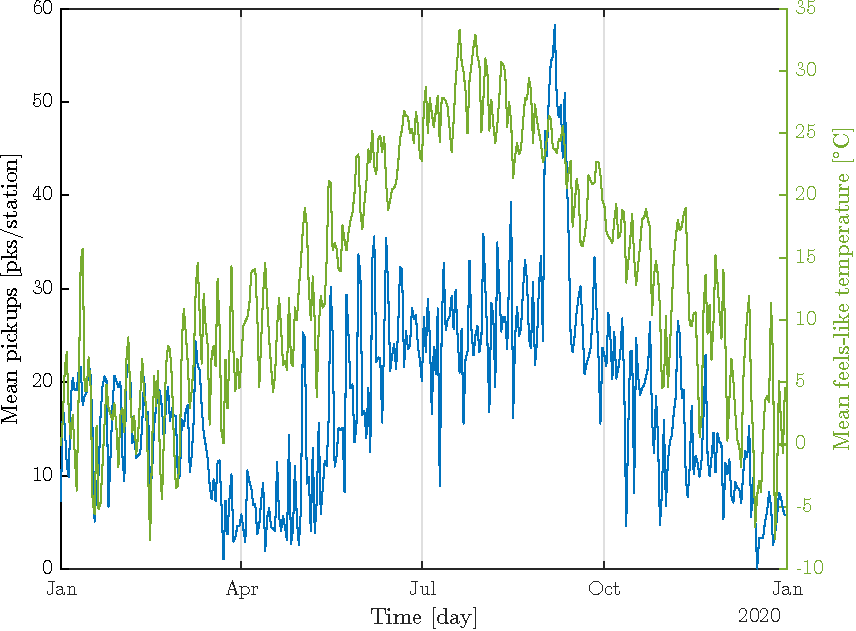
\includegraphics[height=160px]{Images/Dataset description/Chosen/Mean_feels_like_temperature_plot}}\quad
	\subfigure[]{\label{Rain_plot_box}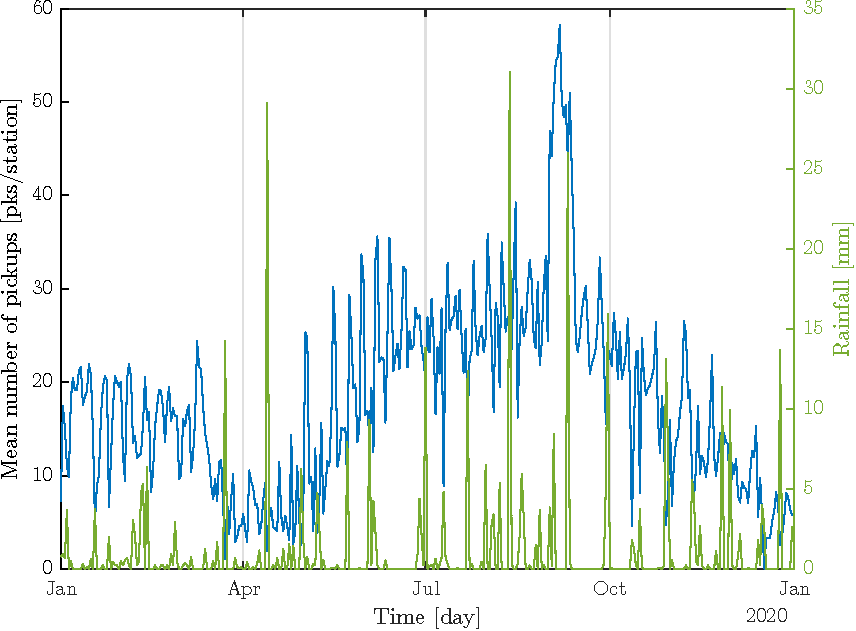
\includegraphics[height=160px]{Images/Dataset description/Chosen/Rainfall_plot}}\quad
	\subfigure[]{\label{T_box}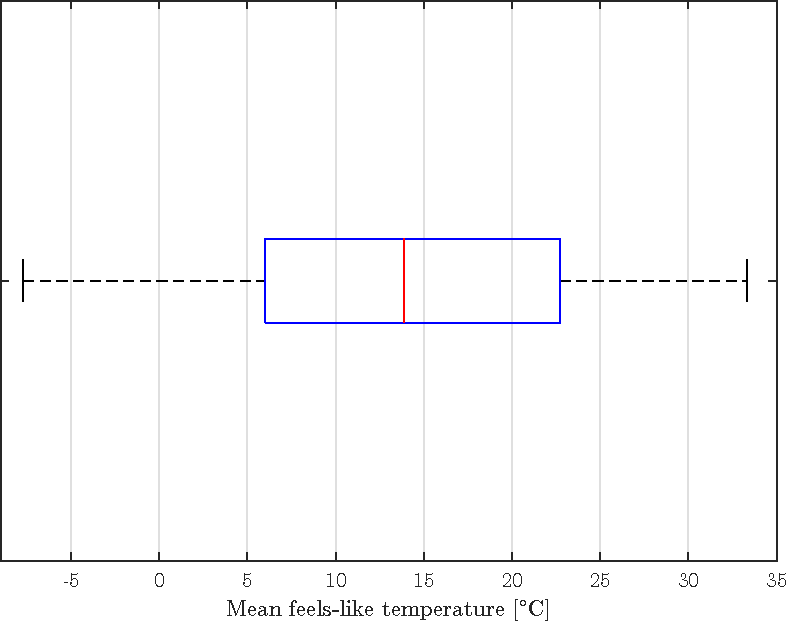
\includegraphics[height=160px]{Images/Dataset description/Chosen/Mean_feels_like_temperature_box}}\quad
	\subfigure[]{\label{Rain_box}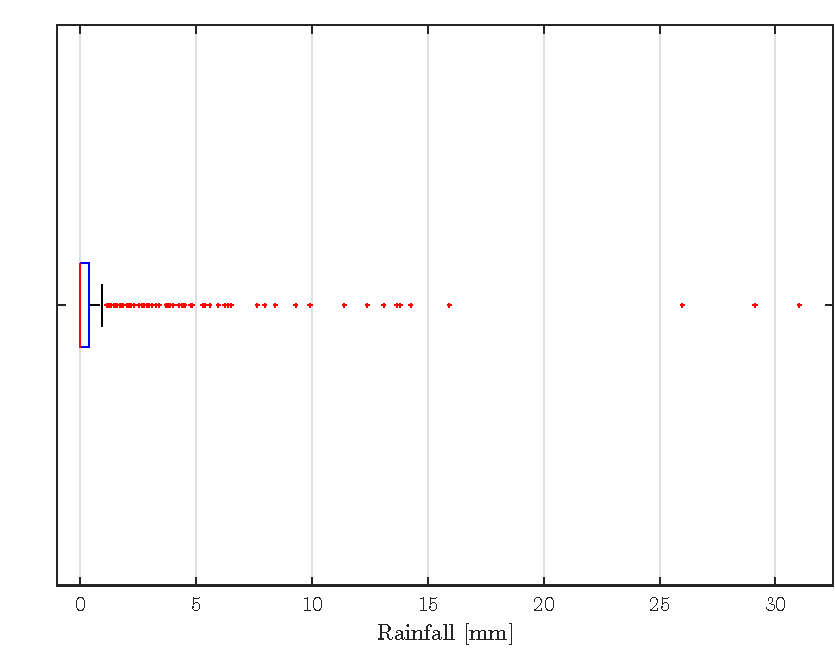
\includegraphics[height=160px]{Images/Dataset description/Chosen/Rainfall_box}}\quad
	\subfigure[]{\label{Cloud_box}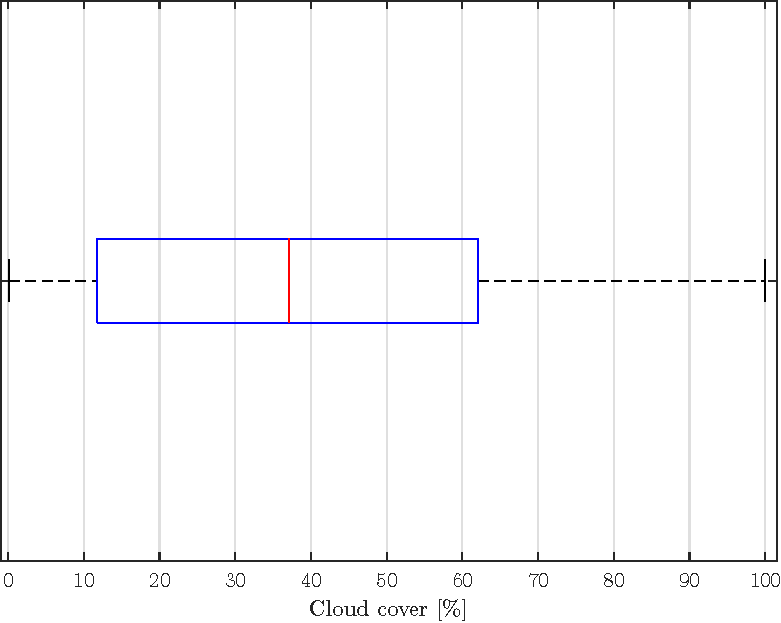
\includegraphics[height=160px]{Images/Dataset description/Chosen/Cloud_cover_box}}\quad
	\subfigure[]{\label{UV_box}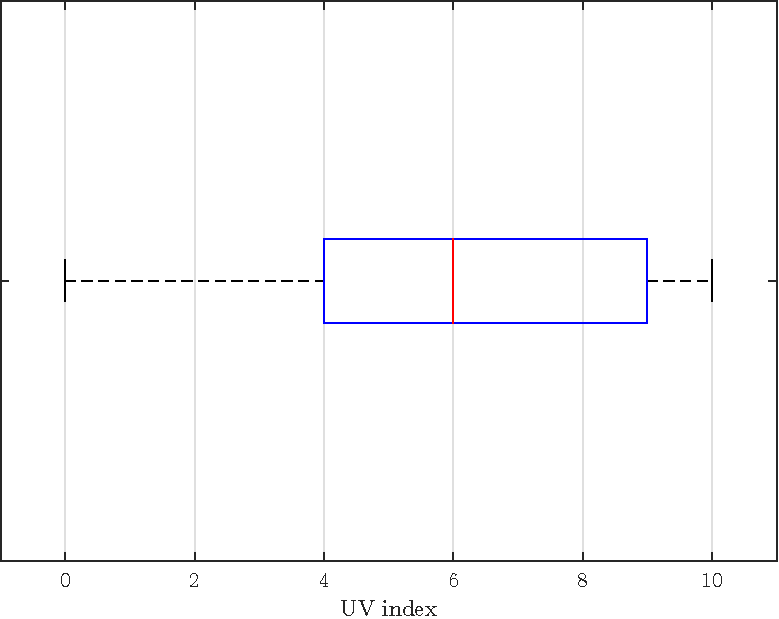
\includegraphics[height=160px]{Images/Dataset description/Chosen/UV_index_box}}\quad
	\caption{On the top left and right, there is the trend of two bike sharing variables, the pickups per station in blue and the average trip duration in dotted red line. On bottom there is the trend of two weather variables in green line, on left is indicated the average feels-like temperature, on right there is the rainfall. The light red patch describes the lockdown period. It is easy to observe that the weather variables have a strong influence, in particular the temperature has a positive effect on the rentals, on the contrary the amount of rainfall has a negative impact. Unfortunately the lockdown breaks these considerations, probably because many people didn't have the possibility to rent a bike}
\end{figure}

\subsection{Other data}
As already mentioned, we hypothesize that some events may influence the demand for bike rentals, especially the presence of lockdowns or the presence of public holidays. So we have defined the following binary dummy variables:
\begin{itemize}
	\item \textbf{lockdown}: this is equal to \num{1} if there are restrictions in New York City, due to Covid and \num{0} if there are none;
	\item \textbf{holidays}: is equal to \num{1} when it is Sunday or when there is a public holiday, \num{0} on the remaining days.
\end{itemize}

\begin{figure}[h!]
	\centering
	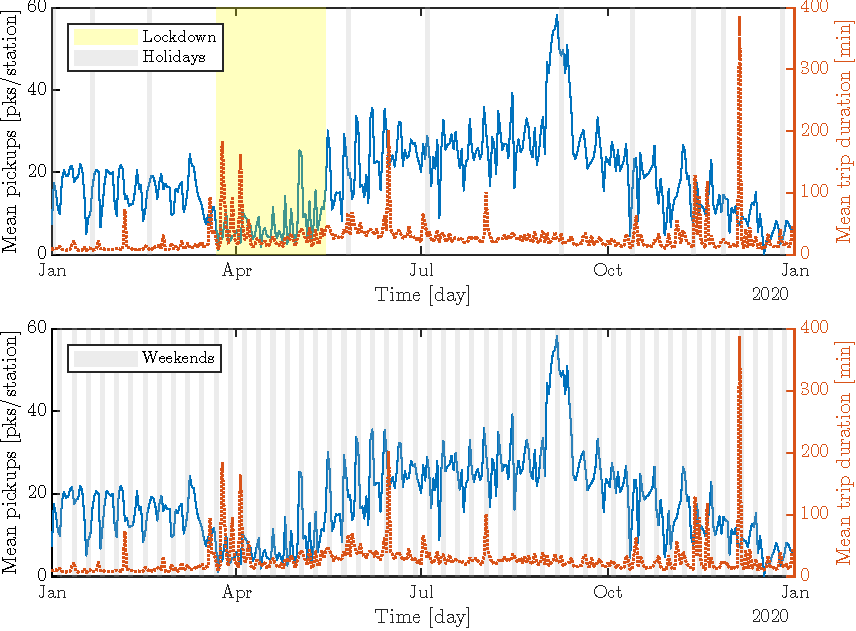
\includegraphics[height = 200px]{Images/Dataset description/Chosen/Trend}
\end{figure}